\section{Experimental Setup}\label{sec:experimentalSetup}

The goal of this research is to build an in-depth understanding about
the performance of the \mas for detecting malware. To this
end, we conduct our research using a dataset of repackaged apps one order of magnitude
larger than previous studies~\cite{DBLP:conf/wcre/BaoLL18,DBLP:journals/jss/CostaMMSSBNR22}. Altogether, our
aim is to answer the following research questions:

\begin{enumerate}[(RQ1)]
\item \rqa
%\item \rqb
\item \rqc
\item \rqd  
\end{enumerate}

In this section, we describe our study settings. First, we present how we mined the samples of Android apps that we
use as a dataset for our study (Section~\ref{sec:dataset}).  Then, we describe the data
collection and data analysis procedures in Sections~\ref{sec:dataCollectionProc} and~\ref{sec:dataAnalysisProc}.


\subsection{Malware Dataset}\label{sec:dataset}


\fh{Our experiment aim to compute if an app pair from a given sample is a repackaged from respective original app. To answer this question, we should run our infrastructure on a representative dataset to estimate \mas precision. This dataset also should be \textit{labeled}, i.e., the interest characteristic of each app, like malware family, should be know beforehand.}

\fh{Figure~\ref{fig:dataset} present the methodology used to extract the dataset for our study. We start with an original dataset containing 15,297 pairs of original/repackaged Android apps~\cite{DBLP:journals/tse/LiBK21}. This original dataset
has been curated using automatic procedures that mine repackaged apps from the Androzoo repository~\cite{DBLP:conf/msr/AllixBKT16}. From this original dataset, we curated a random sample of 5,700 pairs. However, among these 5,700 app pairs, some samples could not be successfully instrumented by DroidFax~\cite{DBLP:conf/icsm/CaiR17a}, or fail to install on the emulator due to compatibility issues with the SDK. After removing incompatible apps, we are left 2,319 samples. To build our final dataset (hereafter \cds), we queried the \vt repository to find out, which app pairs the original app have not been labeled as a malware. \vt is a well-known mechanism for scanning software assets (such as Android apps) using more than 60 anti-virus engines~\cite{DBLP:journals/ese/KhanmohammadiEH19}. In the end, we are left with our \cds of \apps apps which we use for this study. In our research, we also consider a small dataset (hereafter \sds) used in previous studies}~\cite{DBLP:conf/wcre/BaoLL18,DBLP:journals/jss/CostaMMSSBNR22}.

 \begin{figure}
  \includegraphics[width=\columnwidth]{images/dataset.pdf}
  \caption{Malware samples in the Complete Datasets.}
  \label{fig:dataset}
\end{figure}



%starting from an initial sample of 3344 repackaged pairs of apps available in AndroZoo~\cite{DBLP:conf/msr/AllixBKT16}.
%We do not use any particular criteria for selecting the initial sample.
%Nonetheless, due to compatibility issues we found---either during the instrumentation phase (using DroidFax) or during the execution
%phase using the Android emulator---we end-up with our final dataset (hereafter \cds) that contains \apps pairs of
%repackaged apps (36\% of the initial subset repackaged apps).
%\fh{At this paragraph I change the term set to Subset since 3344 is a subset of 15.000 repackage pair}

%\kn{This whole part about Virustotal needs a bit more elaboration. Ideally, including a citation explaining why we go for this additional method of classifying whether something as a malware or not. Since we already start with the app pairs, we sort of already know the malicious and benign version right? }
We also queried the \vt repository to find out which repackaged apps in our
dataset have been indeed labeled as a malware.
%, and we took this decision since the output of \vt can change over time~\cite{vt-label}.\fh{Here I inserted a litle discription of
% VT and inserted some reference}
%(\kn{two out of how many antiviruses are included by Virustotal}). 
According to \vt, in the \sds (102 pairs),
69 of the repackaged apps (67.64\%) have been identified as a malware by at least two
\ses. Here we only consider that a repackaged version of an app is a malware if \vt reports that at least
two \ses identify a malicious behavior within the asset. This is in accordance with previous research~\cite{vt-label,DBLP:journals/ese/KhanmohammadiEH19}. Conversely, considering the \cds, at least two \se identified \malwares out of the \apps repackaged apps as malware (\malwaresP\%).

Classifying malware into different categories is a common practice. For instance, Android malware can be classified into categories
like riskware, trojan, adware, etc. Each category might be further specialized in several malware families, depending of its
characteristics and atack strategy---e.g, steal network info (IP, DNS, WiFi), collect phone info,
collect user contacts, send/receive SMS, and so on~\cite{DBLP:conf/iccns/RahaliLKTGM20}.
According to the
\avt~\cite{avclass2-paper}, the malware samples in the \sds come from $17$ different families---most of them from the Kuguo (49.27\%) and Dowgin (17.39\%) families.
Our \cds, besides a large sample of repackaged apps (\apps in total), it
comprises 44 families of malware we collected using the \avt---most
of them from the Gappusin (60.2\%) family.

We also characterize our dataset according to the similarity
between the original and repackaged versions of the apps, using the  
SimiDroid tool~\cite{DBLP:conf/trustcom/0029BK17}. SimiDroid quantifies the similarity
based on (a) the methods that are either identical or similar in both versions of the apps (original and repackaged versions),
(b) methods that only appear in the repackaged version of the apps (new methods), and (c) methods that only appear in the
original version of the apps (deleted methods).

Our \cds has an average similarity score of 93.37\%---with the follow distribution {\color{red}(27 of
app pairs have a similarity score of less than 25\%, 18 of app pairs
between 25\% and 50\%,  55 of the apps between 50\% and 75\%,
and 1607 of the apps with more than 75\%). The \sds presents a lowest
similarity index average (89.41\%)}. 


\fh{Lastly, we also explored all sensitive APIs called by samples from our dataset. This brought to the light the most frequently abused sensitive APIs that appear in the repackaged, malicious version of our samples. We observed that when executed all samples from \cds, malicious app version injected $138$ sensitive APIs distinct at least one time (from our list of 261 sensitive APIs), whereas Previous studies~\cite{DBLP:conf/wcre/BaoLL18,DBLP:journals/jss/CostaMMSSBNR22} got the most of 101 inserts. The sensitive API that is abused the most by repackaged apps from our dataset is \textbf{java.lang.reflect.Field: java.lang.Object get(java.lang.Object)}. Reflection is an API that can be used to modify the behavior of methods, classes, and interfaces at runtime. Malicious code frequently may use these APIs, or other to help in its attempt to compromise security in the system. Table~\ref{tab:APIused} presents the list of the most frequent sensitive APIs injected at malicious version from our dataset.}




\begin{table*}[ht]
\caption{Sensitive APIs more used by repackage apps.}
\centering
  \begin{tabular}{lc}

    \toprule
    Sensitive API & Occurrences \\
    \midrule
    01 java.lang.reflect.Field: java.lang.Object get(java.lang.Object) &  155 \\
    02 android.net.wifi.WifiInfo: java.lang.String getMacAddress() &  151\\
    03 android.database.sqlite.SQLiteOpenHelper: android.database.sqlite.SQLiteDatabase getWritableDatabase() &  150 \\
    04 android.net.NetworkInfo: android.net.NetworkInfoState getState() &  150 \\
    05 android.net.wifi.WifiManager: android.net.wifi.WifiInfo getConnectionInfo() &  149 \\
    06 android.telephony.TelephonyManager: java.lang.String getSubscriberId() &  147 \\
    07 android.database.sqlite.SQLiteDatabase: android.database.Cursor query(java.lang.String,java.lang.String[],...,java.lang.String) &  146 \\
    08 android.telephony.TelephonyManager: java.lang.String getDeviceId() &  142 \\
   09 android.database.sqlite.SQLiteOpenHelper: android.database.sqlite.SQLiteDatabase getReadableDatabase() &  133 \\
    10 android.net.ConnectivityManager: android.net.NetworkInfo getNetworkInfo(int) &  130\\
    11 android.telephony.TelephonyManager: java.lang.String getNetworkOperator() &  127\\
    12 android.net.NetworkInfo: java.lang.String getTypeName() &  125\\
    13 java.lang.reflect.Field: int getInt(java.lang.Object) &  124 \\
    14 android.telephony.TelephonyManager: java.lang.String getNetworkOperatorName() &  123 \\
    .&  .\\
    .&  .\\
    .&  .\\
    137 java.lang.ClassLoader: java.lang.Class loadClass(java.lang.String,boolean) & 1 \\
    138 java.lang.reflect.Constructor: java.lang.reflect.Type[] getGenericExceptionTypes() & 1 \\

\hline
\end{tabular}
\label{tab:APIused}
\end{table*}

%%  \end{tabular}
%%  %\end{small}
%%  \label{tab:APIused}
%% \end{table*}
%\end{landscape}











It is important to highlight that our sample comes
from different Android app stores. Most of our repackage apps come from a non-official
Android app store, Anzhi~\cite{anzhi}. However some repackaged apps also come from the
official Android app store, Google Play.


%\begin{figure}[ht]
%\centering
%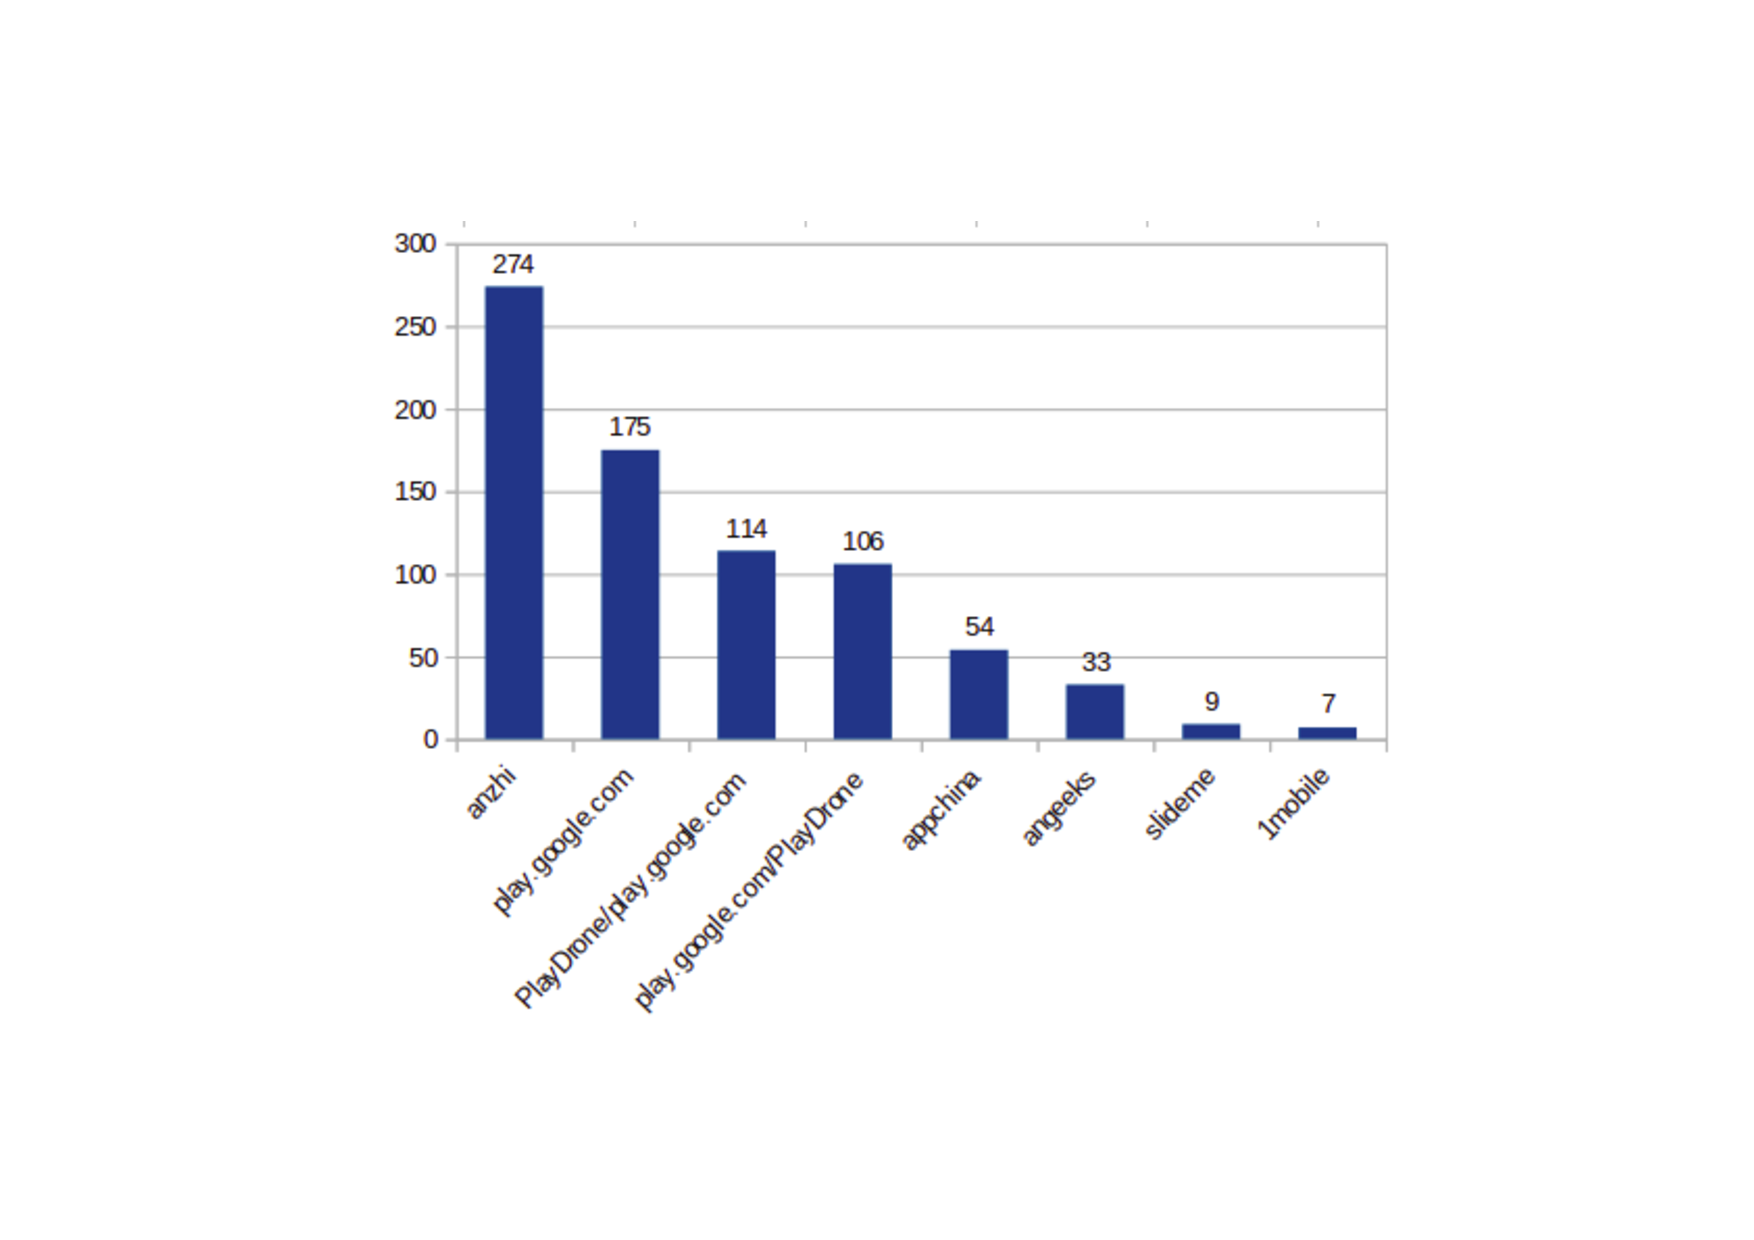
\includegraphics[scale=0.43]{images/stores.pdf}
%\caption{Markets where malware was discovered.}
% \label{fig:stores}
%\end{figure}


\subsection{Data Collection Procedures} \label{sec:dataCollectionProc}

We take advantage of the DroidXP infrastructure~\cite{DBLP:conf/scam/CostaMCMVBC20}
for data collection. DroidXP allows researchers to compare 
test case generation tools in terms of malicious app behaviors identification, using the \mas. Although the comparison of test
case generation tools is not the goal of this paper, DroidXP
was still useful for automating the following steps of our study.


\begin{enumerate}[S1]
 \item \textbf{Instrumentation}: In the first step,
we configure DroidXP to instrument all pairs of apps in our dataset.
Here, we instrument both versions of the apps (as APK files) to collect relevant information during their execution. Under the hood, DroidXP leverages
DroidFax~\cite{DBLP:conf/icsm/CaiR17a} to instrument the apps and collect static
information about them. To improve the performance across multiple executions,
this phase executes only once for each version of the apps in our dataset.

\item \textbf{Execution}: In this step, DroidXP first installs the (instrumented) version of the APK files in the Android emulator we use in our experiment (API 28) and then starts a test case generation tool for executing both apps version (original and repackage). We execute the apps via DroidBot~\cite{DBLP:conf/icse/LiYGC17}, mostly because previous works report the best accuracy of the sandboxes built using the \mas and the DroidBot as test case generation tool. To also ensure that each execution gets the benefit of running on a fresh Android instance without biases that could stem out of history, DroidXP wipes out all data stored on the emulator that has been collected from previous executions.


\item \textbf{Data Collection}: During the execution of the instrumented apps, we collect all relevant information (such as calls to sensitive APIs, test coverage metrics, and so on). We use this information to analyse the performance of the \mas for detecting malicious behavior.
\end{enumerate}

\subsection{Data Analysis Procedures} \label{sec:dataAnalysisProc}

\fh{After running the dynamic analysis via DroidBot, our infrastructure produces
new datasets with the sensitive APIs that both app versions call during their execution. The set of sensitive APIs used at this work was defined in the AppGuard framework~\cite{DBLP:conf/esorics/BackesGHMS13}, which was based on the mapping from sensitive APIs to permissions proposed by Song et al.~\cite{DBLP:conf/ccs/FeltCHSW11}}


We consider that a test
generation tool, in our case, DroidBot, builds a sandbox that labels a repackaged version
of an app as a malware if there is at least one call to a sensitive APIs that (a) was observed
while executing the repackaged version of the app and that (b) was not observed while
executing the original version of the same app. 
If the set of sensitive methods that only the repackaged version of an app calls is empty,
we conclude that the sandbox does not label the repackaged version of an app as a malware. We triangulate
this information with the outputs of \vt, which might lead to one of the following
situations:

\begin{itemize}
\item {\bf True Positive}. The \mas labels a repackaged version as a malware and, according to
  \vt, at least two \ses label the asset as a malware.
  
\item {\bf True Negative}. The \mas does not label a repackaged version as a malware and,
  according to \vt, at most one \se labels the asset as a malware. 

\item {\bf False Positive}. The \mas labels a repackaged version as a malware and, according to
  \vt, at most one \se labels the asset as a malware.

\item {\bf False Negative}. The \mas does not label a repackaged version as a malware, and
  according to \vt, at least two \ses label the asset as a malware.
\end{itemize}

We use basic statistics (average, median, standard deviation) to identify the
accuracy of the \mas for malware classification, in both
datasets we use in our research---i.e., the \sds
with 102 pairs of apps and our \cds with
\apps pairs. We use the Spearman Correlation~\cite{spearman-correlation} method and
Logistic Regression~\cite{statistical-learning} to understand the strengths of
the associations between the similarity index of a
malware with the \mas accuracy---that is,
if the approach was able to correctly classify an asset as malware. We also use existing tools to reverse engineer a sample of repackaged
apps in order to better understand (the lack of) accuracy
of the \mas.



%\fh{I removed the item C of this section that talk about hardware and execution time.}

\subsection{Environment Configuration}\label{sec:hardware}

%\todo[inline]{RB: later, if we need space, we can safely comment this section out.}

We deployed our experiment on a 32-Core, AMD EPYC 7542 CPU, 512 GB RAM, storage Samsung SSD 970 EVO 1TB machine running a 64-bit Debian GNU/Linux 11. We also configured our emulator to run all selected apps on Google Android version 9.0, API 28, 512M SD Card, 7GB internal storage, with X86 ABI image.

For our study, we configured DroidXP to run each of the \apps app pairs using DroidBot for 3 minutes. To mitigate noise, we repeated the full process 3 times,  which took around 513 machine hours in total. Although it was possible to run more than 10 emulators in parallel on one physical machine, to avoid any interference resulting from context switching within the operating system, we chose to run one emulator at a time. Hence, all processes took around 27 days, 23 days for experiment execution and additional 4 days for environment configuration.%\rb{I don't know if the following is relevant\ldots} 

